\begin{figure}[t]
\centering
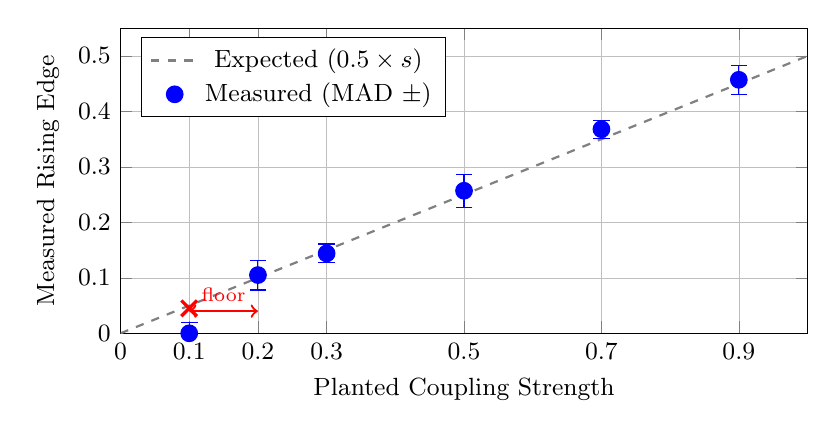
\begin{tikzpicture}
\begin{axis}[
  width=0.85\textwidth,
  height=0.45\textwidth,
  xlabel={Planted Coupling Strength},
  ylabel={Measured Rising Edge},
  xmin=0, xmax=1.0,
  ymin=0, ymax=0.55,
  xtick={0,0.1,0.2,0.3,0.5,0.7,0.9},
  xticklabels={0,0.1,0.2,0.3,0.5,0.7,0.9},
  ytick={0,0.1,0.2,0.3,0.4,0.5},
  grid=both,
  grid style={line width=.1pt, draw=gray!30},
  major grid style={line width=.2pt,draw=gray!50},
  legend pos=north west,
  legend style={font=\small},
  tick label style={font=\small},
  label style={font=\small},
]

% Expected line: y = 0.5 * x
\addplot[domain=0:1, dashed, gray, thick] {0.5*x};
\addlegendentry{Expected ($0.5 \times s$)}

% Measured points
\addplot[only marks, mark=*, mark size=3pt, color=blue,
  error bars/.cd, y dir=both, y explicit]
coordinates {
  (0.1, 0) +- (0,0.019)
  (0.2, 0.105) +- (0,0.027)
  (0.3, 0.144) +- (0,0.017)
  (0.5, 0.257) +- (0,0.030)
  (0.7, 0.368) +- (0,0.016)
  (0.9, 0.457) +- (0,0.026)
};
\addlegendentry{Measured (MAD $\pm$)}

% Detection floor annotation
\draw[<->, red, thick] (axis cs:0.1,0.04) -- (axis cs:0.2,0.04);
\node[red, font=\scriptsize, above] at (axis cs:0.15,0.04) {floor};

% Not detected marker
\addplot[only marks, mark=x, mark size=4pt, color=red, very thick]
coordinates {(0.1, 0.045)};

\end{axis}
\end{tikzpicture}
\caption{Detection sensitivity at noise $\sigma = 0.02$ (linear
coupling). Blue circles: measured rising edge with MAD error bars.
Dashed line: expected edge ($s \times 0.5$). Red $\times$: not
detected (below CFAR threshold). Measurement error consistently
below 5\%. Detection floor lies between coupling 0.1 and 0.2.}
\label{fig:sensitivity}
\end{figure}
